% Created 2024-07-07 Sun 22:03
% Intended LaTeX compiler: xelatex
\documentclass[a4paper,11pt,twoside]{article}
\usepackage{graphicx}
\usepackage{longtable}
\usepackage{wrapfig}
\usepackage{rotating}
\usepackage[normalem]{ulem}
\usepackage{amsmath}
\usepackage{amssymb}
\usepackage{capt-of}
\usepackage{hyperref}
\usepackage{libertine} \usepackage{amsmath}
\usepackage[width=200.00mm, height=240.00mm, left=3cm, right=3cm, top=3 cm, bottom=3cm]{geometry}
\usepackage{graphicx}
\graphicspath{ {./images/} }
\usepackage{multicol}
\author{Ryan P. Lynch}
\date{\today}
\title{Program 1A}
\hypersetup{
 pdfauthor={Ryan P. Lynch},
 pdftitle={Program 1A},
 pdfkeywords={},
 pdfsubject={},
 pdfcreator={Emacs 29.3 (Org mode 9.6.24)}, 
 pdflang={English}}
\usepackage{biblatex}

\begin{document}

\maketitle

\section*{Illustration}
\label{sec:org7caec53}
\begin{multicols}{2}
\noindent
We start with only the parent process\\
\\
\\
\\
\\
Execute pipe twice to create the file descriptors we need\\
\\
\\
\\
\\
\\
\\
\\
\\
\\
Fork the parent process, copying file descriptors\\
\\
\\
\\
\\
\\
\\
\\
\\
\\
Fork the child process, copying file descriptors\\
\vfill\null
\columnbreak
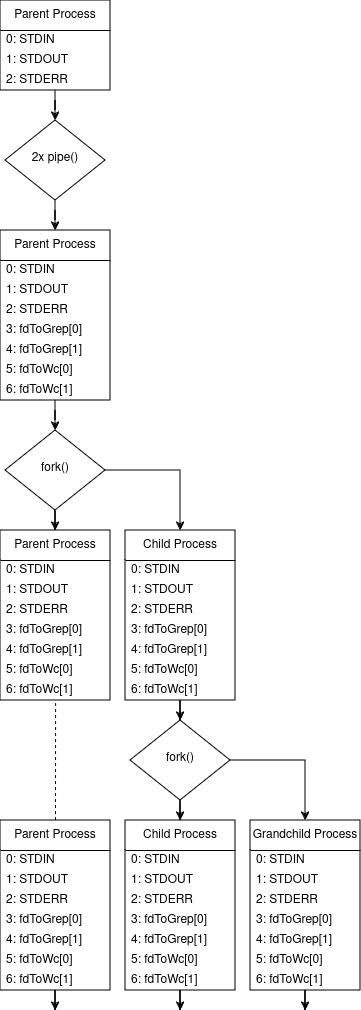
\includegraphics[width=0.42\textwidth]{flow-diagram.drawio0}
\end{multicols}
\begin{multicols}{2}
\\
\\
\\
\\
\\
\noindent
Duplicate the file descriptors to the Standard Out/In of their processes\\
\\
\\
\\
\\
\\
\\
\\
\\
\\
\\
\\
Close the file descriptors we no longer need
\\
\\
\\
\\
\\
\\
\\
\\
\\
Execute ps command, the child process is waiting for this to finish. Sends results through Standard Out and pipes into Standard In of child process
\\
\\
\\
\\
\\
\\
Execute grep command, the parent process is waiting for this to finish. Sends results through Standard Out and pipes into Standard In of parent process
\\
\\
\\
\\
\\
\\
\\
\\
Execute wc command. Sends results through Standard Out.
\vfill\null
\columnbreak
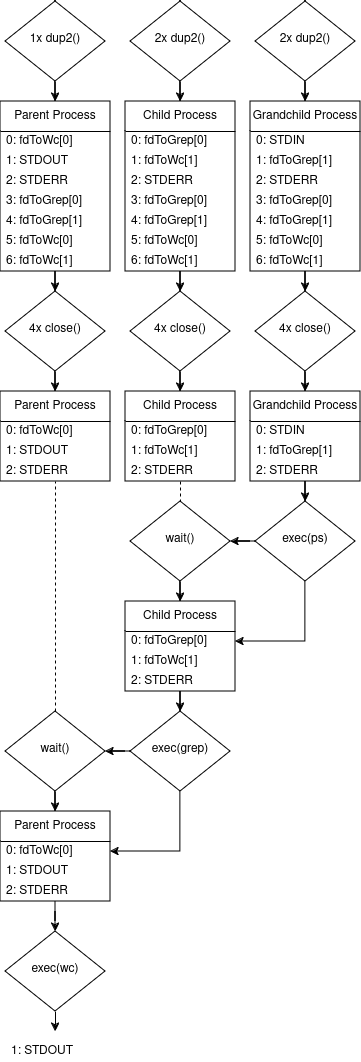
\includegraphics[width=0.5\textwidth]{flow-diagram.drawio}
\end{multicols}
\section*{Compile and Execution}
\label{sec:orge5dcff9}
The screenshot below is proof that I compiled and ran the homework assignment on the UWB lab machines.
\begin{center}
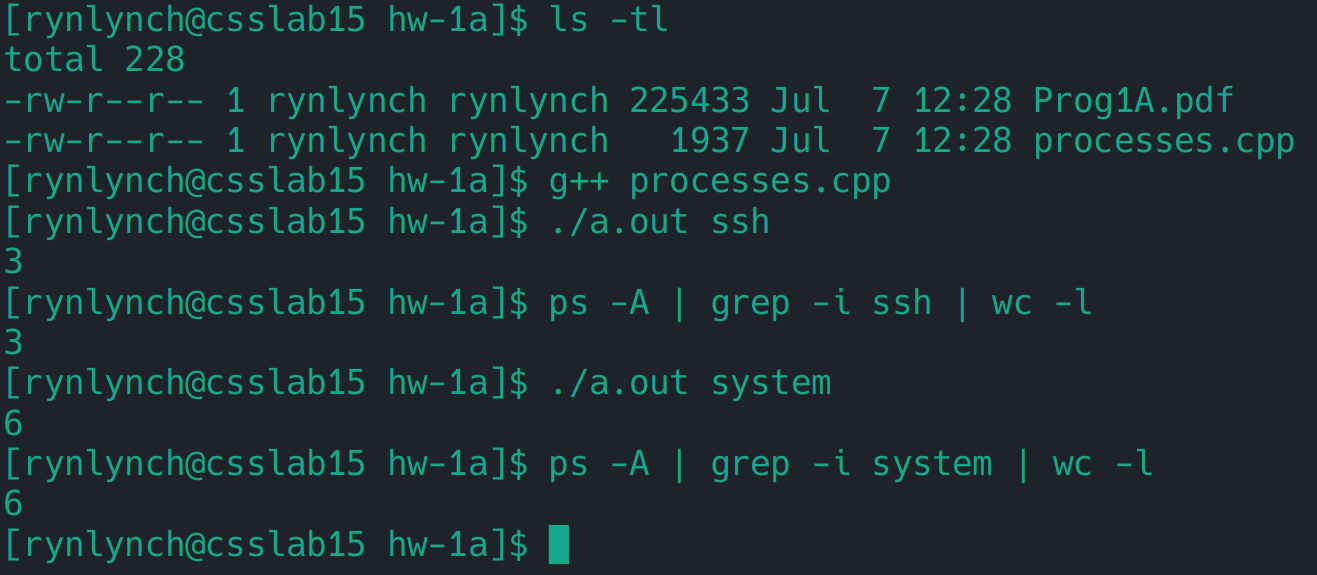
\includegraphics[width=.9\linewidth]{./images/compile-and-execution.png}
\end{center}
This also shows the program returning the same value as the equivalent commands on the CLI
\begin{verbatim}
ps -A | grep -i ssh | wc -l
\end{verbatim}
\end{document}
